% для компиляции в lualatex!!
%\documentclass[12pt, a4paper]{article}
\documentclass[12pt, a4paper]{disser}
\usepackage[english,russian]{babel}
\usepackage[warn]{mathtext}
%\usepackage[T2A]{fontenc}
%\usepackage[utf8]{inputenc}

\usepackage{xecyr} % Продукт Вашего покорного слуги ;)

%\setmainfont{DejaVu Serif}
\setmainfont{Liberation Serif}

\usepackage{color}
\usepackage{amssymb,amsmath}
\usepackage{graphicx}
\usepackage{multicol}
\usepackage{csvtools}

\textheight=24cm           % высота текста
\textwidth=16cm            % ширина текста
\oddsidemargin=0pt         % отступ от левого края
\topmargin=-1.5cm          % отступ от верхнего края
\parindent=24pt            % абзацный отступ
\parskip=0pt               % интервал между абзацами
\tolerance=2000            % терпимость к "жидким" строкам
\flushbottom               % выравнивание высоты страниц
%\def\baselinestretch{1.5} % печать с большим интервалом

%\title{}
%\author{\copyright~~С.А.~Назарова \thanks{e-mail:~sophia.nazarova@gmail.com}}
%\date{}


\begin{document}

	\section{Численность {\it Macoma balthica}}
	\subsection{Белое море}
Данные по обилию маком в Кандалакшском заливе Белого моря получены для $10$ участков, всего 140 пространственно-временных точек оценки.
Средняя численность {\it M.~balthica} была представлена в диапазоне от $10$ (о.~Горелый) до $8500$~экз./м$^2$(Западная Ряшкова салма) (табл. \ref{tab:mean_N_White}).
	\begin{footnotesize}
	\begin{longtable}{|p{2cm}|p{3cm}|p{1cm}|p{2cm}|p{1.5cm}|p{1cm}|*{3}{c|}}
	\caption{Средняя численность {\it Macoma balthica} на различных участках Белого моря}\label{tab:mean_N_White}\\
	\hline
	Район & Участок & год & ма\-ре\-ографи\-ческий уровень & число повторностей & площадь учета & $N$, экз./м$^2$ & $S_x$  & $D, \%$ 
	\\ \hline \endfirsthead
	\hline
	\multicolumn{9}{|c|}{продолжение таблицы \ref{tab:mean_N_White}} \\ \hline
	Район & Участок & год & ма\-ре\-ографи\-ческий уровень & число повторностей & площадь учета & $N$, экз./м$^2$ & $S_x$  & $D, \%$ 
	\\ \hline \endhead
	\hline 
	\multicolumn{9}{|c|}{продолжение таблицы \ref{tab:mean_N_White} на следующей странице}
	\\ \hline \endfoot
	 \endlastfoot
	г. Чупа & б. Клющиха & 2006 & СГЛ & 10 & 1/20 & 444 & 53,7 & 12
		\\ \cline{3-9}
		 &  & 2006 & НГЛ & 10 & 1/20 & 362 & 26,4 & 7
		\\ \cline{3-9}
		 &  & 2006 & ВСЛ & 10 & 1/20 & 1136 & 55,4 & 5
		\\ \cline{2-9}
		 & Сухая салма & 2006 & СГЛ & 10 и & 2/20 & 1165 & 169,3 & 15
		\\ \cline{3-9}
		 &  & 2006 & НГЛ & 5 & 1/20 & 1132 & 82,6 & 7
		\\ \cline{3-9}
		 &  & 2006 & НГЛ, пояс зостеры & 5 & 1/20 & 992 & 174,4 & 18
		\\ \cline{2-9}
		 & б. Лисья & 2006 & СГЛ & 10 & 1/20 & 1346 & 209,8 & 16
		\\ \cline{3-9}
		 &  & 2006 & НГЛ & 10 & 1/20 & 2832 & 277,8 & 10
		\\ \cline{3-9}
		 &  & 2006 & ВСЛ & 10 & 1/20 & 1006 & 159,8 & 16
		\\ \cline{2-9}
		 & пр. Подпахта & 2006 & СГЛ & 10 & 1/20 & 688 & 145,2 & 21
		\\ \cline{3-9}
		 &  & 2006 & НГЛ & 10 & 1/20 & 372 & 57,9 & 16
		\\ \hline
	Лувеньга & материковая литораль, Лувеньга & 1992 & верхний пляж & 7 & 1/30 & 94 & 35,5 & 38
		\\ \cline{4-9}
		 &  & 1992 & пояс фукоидов & 5 & 1/30 & 114 & 55,6 & 49
		\\ \cline{4-9}
		 &  &  & пояс зостеры & 5 & 1/30 & 222 & 103,3 & 47
		\\ \cline{4-9}
		 &  &  & нижний пляж & 3 & 1/30 & 560 & 457,1 & 82
		\\ \cline{3-9}
		 &  & 1993 & верхний пляж & 4 & 1/30 & 413 & 127,5 & 31
		\\ \cline{4-9}
		 &  &  & пояс фукоидов & 5 & 1/30 & 336 & 120,9 & 36
		\\ \cline{4-9}
		 &  &  & пояс зостеры & 6 & 1/30 & 405 & 80,0 & 20
		\\ \cline{4-9}
		 &  & & нижний пляж & 5 & 1/30 & 354 & 77,3 & 22
		\\ \cline{3-9}
		 &  & 1994 & верхний пляж & 5 & 1/30 & 462 & 179,1 & 39
		\\ \cline{4-9}
		 &  &  & пояс фукоидов & 6 & 1/30 & 745 & 220,6 & 30
		\\ \cline{4-9}
		 &  &  & пояс зостеры & 6 & 1/30 & 765 & 112,7 & 15
		\\ \cline{4-9}
		 &  &  & нижний пляж & 3 & 1/30 & 930 & 170,6 & 18
		\\ \cline{3-9}
		 &  & 1995 & верхний пляж & 4 & 1/30 & 908 & 222,3 & 24
		\\ \cline{4-9}
		 &  &  & пояс фукоидов & 5 & 1/30 & 1134 & 269,7 & 24
		\\ \cline{4-9}
		 &  &  & пояс зостеры & 5 & 1/30 & 660 & 117,7 & 18
		\\ \cline{4-9}
		 &  &  & нижний пляж & 6 & 1/30 & 685 & 154,8 & 23
		\\ \cline{3-9}
		 &  & 1996 & верхний пляж & 4 & 1/30 & 698 & 257,0 & 37
		\\ \cline{4-9}
		 &  &  & пояс фукоидов & 6 & 1/30 & 770 & 214,9 & 28
		\\ \cline{4-9}
		 &  &  & пояс зостеры & 4 & 1/30 & 645 & 71,9 & 11
		\\ \cline{4-9}
		 &  &  & нижний пляж & 6 & 1/30 & 870 & 68,8 & 8
		\\ \cline{3-9}
		 &  & 1997 & верхний пляж & 3 & 1/30 & 620 & 130,0 & 21
		\\ \cline{4-9}
		 &  &  & пояс фукоидов & 6 & 1/30 & 720 & 265,6 & 37
		\\ \cline{4-9}
		 &  &  & пояс зостеры & 5 & 1/30 & 702 & 70,7 & 10
		\\ \cline{4-9}
		 &  &  & нижний пляж & 6 & 1/30 & 880 & 97,0 & 11
		\\ \cline{3-9}
		 &  & 1998 & верхний пляж & 4 & 1/30 & 2130 & 623,9 & 29
		\\ \cline{4-9}
		 &  &  & пояс фукоидов & 6 & 1/30 & 2750 & 820,0 & 30
		\\ \cline{4-9}
		 &  &  & пояс зостеры & 5 & 1/30 & 2424 & 437,1 & 18
		\\ \cline{4-9}
		 &  &  & нижний пляж & 5 & 1/30 & 1182 & 239,0 & 20
		\\ \cline{3-9}
		 &  & 1999 & верхний пляж & 3 & 1/30 & 7240 & 5833,7 & 81
		\\ \cline{4-9}
		 &  &  & пояс фукоидов & 6 & 1/30 & 3895 & 1354,6 & 35
		\\ \cline{4-9}
		 &  &  & пояс зостеры & 6 & 1/30 & 2405 & 498,8 & 21
		\\ \cline{4-9}
		 &  &  & нижний пляж & 5 & 1/30 & 2328 & 623,8 & 27
		\\ \cline{3-9}
		 &  & 2000 & верхний пляж & 2 & 1/30 & 2640 & 870,0 & 33
		\\ \cline{4-9}
		 &  &  & пояс фукоидов & 4 & 1/30 & 2760 & 373,1 & 14
		\\ \cline{4-9}
		 &  & & пояс зостеры & 5 & 1/30 & 2562 & 721,0 & 28
		\\ \cline{4-9}
		 &  &  & нижний пляж & 4 & 1/30 & 2018 & 394,3 & 20
		\\ \cline{3-9}
		 &  & 2002 & верхний пляж & 3 & 1/30 & 1360 & 401,5 & 30
		\\ \cline{4-9}
		 &  &  & пояс фукоидов & 3 & 1/30 & 3250 & 337,8 & 10
		\\ \cline{4-9}
		 &  &  & пояс зостеры & 4 & 1/30 & 2498 & 952,6 & 38
		\\ \cline{4-9}
		 &  &  & нижний пляж & 2 & 1/30 & 810 & 240,0 & 30
		\\ \cline{3-9}
		 &  & 2004 & верхний пляж & 3 & 1/30 & 2800 & 1066,6 & 38
		\\ \cline{4-9}
		 &  &  & пояс фукоидов & 4 & 1/30 & 3090 & 889,0 & 29
		\\ \cline{4-9}
		 &  &  & пояс зостеры & 5 & 1/30 & 1818 & 302,6 & 17
		\\ \cline{2-9}
		 & о. Горелый & 1992 & ВГЛ & 7 & 1/30 & 73 & 23,7 & 32
		\\ \cline{4-9}
		 &  &  & СГЛ & 5 & 1/30 & 108 & 9,7 & 9
		\\ \cline{4-9}
		 &  &  & НГЛ & 2 & 1/30 & 50 & 20,0 & 40
		\\ \cline{4-9}
		 &  &  & ноль глубин & 3 & 1/30 & 13 & 3,3 & 25
		\\ \cline{3-9}
		 &  & 1993 & ВГЛ & 3 & 1/30 & 143 & 29,1 & 20
		\\ \cline{4-9}
		 &  &  & СГЛ & 3 & 1/30 & 480 & 11,5 & 2
		\\ \cline{4-9}
		 &  &  & НГЛ & 4 & 1/30 & 183 & 34,5 & 19
		\\ \cline{4-9}
		 &  &  & ноль глубин & 3 & 1/30 & 97 & 43,7 & 45
		\\ \cline{3-9}
		 &  & 2004 & ВГЛ & 3 & 1/30 & 2620 & 219,3 & 8
		\\ \cline{4-9}
		 &  &  & СГЛ & 3 & 1/30 & 1700 & 208,8 & 12
		\\ \cline{4-9}
		 &  &  & НГЛ & 3 & 1/30 & 1040 & 176,9 & 17
		\\ \cline{4-9}
		 &  &  & ноль глубин & 3 & 1/30 & 1540 & 60,8 & 4
		\\ \cline{3-9}
		 &  & 2006 & ВГЛ & 3 & 1/30 & 2200 & 353,4 & 16
		\\ \cline{4-9}
		 &  &  & СГЛ & 3 & 1/30 & 1910 & 342,2 & 18
		\\ \cline{4-9}
		 &  &  & НГЛ & 3 & 1/30 & 650 & 87,2 & 13
		\\ \cline{4-9}
		 &  &  & ноль глубин & 3 & 1/30 & 760 & 160,9 & 21
		\\ \cline{3-9}
		 &  & 2007 & ВГЛ & 3 & 1/30 & 1940 & 341,8 & 18
		\\ \cline{4-9}
		 &  &  & СГЛ & 3 & 1/30 & 1990 & 449,8 & 23
		\\ \cline{4-9}
		 &  &  & НГЛ & 3 & 1/30 & 540 & 195,2 & 36
		\\ \cline{4-9}
		 &  &  & ноль глубин & 3 & 1/30 & 660 & 45,8 & 7
		\\ \cline{3-9}
		 &  & 2008 & ВГЛ & 3 & 1/30 & 1100 & 98,5 & 9
		\\ \cline{4-9}
		 &  &  & СГЛ & 3 & 1/30 & 2740 & 125,3 & 5
		\\ \cline{4-9}
		 &  &  & НГЛ & 3 & 1/30 & 1030 & 404,5 & 39
		\\ \cline{4-9}
		 &  &  & ноль глубин & 3 & 1/30 & 740 & 147,3 & 20
		\\ \cline{3-9}
		 &  & 2011 & ВГЛ & 3 & 1/30 & 2000 & 926,0 & 46
		\\ \cline{4-9}
		 &  &  & СГЛ & 3 & 1/30 & 1210 & 216,6 & 18
		\\ \cline{4-9}
		 &  &  & НГЛ & 3 & 1/30 & 1590 & 199,7 & 13
		\\ \cline{4-9}
		 &  &  & ноль глубин & 3 & 1/30 & 1100 & 208,8 & 19
		\\ \cline{2-9}
	 & Эстуарий р.~Лувень\-ги & 1992 & НГЛ & 6 & 1/30 & 55 & 14,8 & 27
		\\ \cline{3-9}
		 &  & 1993 & НГЛ & 6 & 1/30 & 202 & 31,3 & 16
		\\ \cline{3-9}
		 &  & 1994 & НГЛ & 3 и & 3/30 & 777 & 129,9 & 17
		\\ \cline{3-9}
		 &  & 1995 & НГЛ & 3 и & 3/30 & 473 & 44,8 & 9
		\\ \cline{3-9}
		 &  & 1996 & НГЛ & 3 и & 3/30 & 337 & 29,1 & 9
		\\ \cline{3-9}
		 &  & 1997 & НГЛ & 3 и & 3/30 & 213 & 14,5 & 7
		\\ \cline{3-9}
		 &  & 1998 & НГЛ & 3 и & 3/30 & 750 & 15,3 & 2
		\\ \cline{3-9}
		 &  & 1999 & НГЛ & 3 и & 3/30 & 2073 & 633,3 & 31
		\\ \cline{3-9}
		 &  & 2000 & НГЛ & 3 и & 3/30 & 1913 & 86,5 & 5
		\\ \cline{3-9}
		 &  & 2001 & НГЛ & 3 и & 3/30 & 2607 & 139,6 & 5
		\\ \cline{3-9}
		 &  & 2002 & НГЛ & 3 и & 3/30 & 1917 & 209,0 & 11
		\\ \cline{3-9}
		 &  & 2003 & НГЛ & 3 и & 3/30 & 2220 & 235,4 & 11
		\\ \cline{3-9}
		 &  & 2004 & НГЛ & 3 и & 3/30 & 3330 & 315,0 & 9
		\\ \cline{3-9}
		 &  & 2005 & НГЛ & 3 и & 3/30 & 1623 & 161,8 & 10
		\\ \cline{3-9}
		 &  & 2006 & НГЛ & 3 и & 3/30 & 993 & 131,3 & 13
		\\ \cline{3-9}
		 &  & 2007 & НГЛ & 9 & 1/30 & 2547 & 341,8 & 13
		\\ \cline{3-9}
		 &  & 2008 & НГЛ & 3 и & 3/30 & 1683 & 343,5 & 20
		\\ \cline{3-9}
		 &  & 2009 & НГЛ & 3 и & 3/30 & 1860 & 146,4 & 8
		\\ \cline{3-9}
		 &  & 2010 & НГЛ & 3 и & 3/30 & 2057 & 231,5 & 11
		\\ \cline{3-9}
		 &  & 2011 & НГЛ & 9 & 1/30 & 1637 & 60,2 & 4
		\\ \cline{3-9}
		 &  & 2012 & НГЛ & 3 и & 3/30 & 1170 & 23,1 & 2
		\\ \hline
	Северный архипелаг & Западная Ряшкова салма & 1994 & СГЛ & 2 и & 3/30 & 450 & 100,0 & 22
		\\ \cline{3-9}
		 &  & 1995 & СГЛ & 2 и & 3/30 & 490 & 10,0 & 2
		\\ \cline{3-9}
		 &  & 1996 & СГЛ & 2 и & 3/30 & 260 & 130,0 & 50
		\\ \cline{3-9}
		 &  & 1997 & СГЛ & 2 и & 3/30 & 220 & 90,0 & 41
		\\ \cline{3-9}
		 &  & 1998 & СГЛ & 2 и & 3/30 & 755 & 185,0 & 25
		\\ \cline{3-9}
		 &  & 1999 & СГЛ & 2 и & 3/30 & 8530 & 800,0 & 9
		\\ \cline{3-9}
		 &  & 2000 & СГЛ & 2 и & 3/30 & 2910 & 440,0 & 15
		\\ \cline{3-9}
		 &  & 2001 & СГЛ & 2 и & 3/30 & 2515 & 295,0 & 12
		\\ \cline{3-9}
		 &  & 2002 & СГЛ & 2 и & 3/30 & 2690 & 570,0 & 21
		\\ \cline{3-9}
		 &  & 2003 & СГЛ & 2 и & 3/30 & 1930 & 300,0 & 16
		\\ \cline{3-9}
		 &  & 2004 & СГЛ & 2 и & 3/30 & 2355 & 55,0 & 2
		\\ \cline{3-9}
		 &  & 2005 & СГЛ & 2 и & 3/30 & 1825 & 115,0 & 6
		\\ \cline{3-9}
		 &  & 2006 & СГЛ & 2 и & 3/30 & 795 & 165,0 & 21
		\\ \cline{3-9}
		 &  & 2007 & СГЛ & 2 и & 3/30 & 1055 & 185,0 & 18
		\\ \cline{3-9}
		 &  & 2008 & СГЛ & 2 и & 3/30 & 1840 & 460,0 & 25
		\\ \cline{3-9}
		 &  & 2009 & СГЛ & 2 и & 3/30 & 1745 & 65,0 & 4
		\\ \cline{3-9}
		 &  & 2010 & СГЛ & 2 и & 3/30 & 1680 & 460,0 & 27
		\\ \cline{3-9}
		 &  & 2011 & СГЛ & 2 и & 3/30 & 1455 & 535,0 & 37
		\\ \cline{3-9}
		 &  & 2012 & СГЛ & 2 и & 3/30 & 910 & 340,0 & 37
		\\ \cline{2-9}
	 & Южная губа о. Ряшкова & 2001 & ноль глубин & 9 & 1/30 & 1257 & 174,8 & 14
		\\ \cline{3-9}
		 &  & 2002 & ноль глубин & 16 & 1/30 & 1196 & 212,5 & 18
		\\ \cline{3-9}
		 &  & 2003 & ноль глубин & 15 & 1/30 & 1758 & 333,3 & 19
		\\ \cline{3-9}
		 &  & 2004 & ноль глубин & 13 & 1/30 & 1913 & 576,0 & 30
		\\ \cline{3-9}
		 &  & 2005 & ноль глубин & 15 & 1/30 & 860 & 178,0 & 21
		\\ \cline{3-9}
		 &  & 2006 & ноль глубин & 12 & 1/30 & 843 & 203,9 & 24
		\\ \cline{3-9}
		 &  & 2007 & ноль глубин & 15 & 1/30 & 1412 & 387,8 & 27
		\\ \cline{3-9}
		 &  & 2008 & ноль глубин & 10 & 1/30 & 1434 & 333,4 & 23
		\\ \cline{3-9}
		 &  & 2009 & ноль глубин & 15 & 1/30 & 1122 & 198,5 & 18
		\\ \cline{3-9}
		 &  & 2010 & ноль глубин & 15 & 1/30 & 682 & 106,5 & 16
		\\ \cline{3-9}
		 &  & 2011 & ноль глубин & 15 & 1/30 & 364 & 151,5 & 42
		\\ \cline{3-9}
		 &  & 2012 & ноль глубин & 15 & 1/30 & 142 & 39,1 & 28
		\\ \cline{2-9}
	 & о. Ломнишный & 2007 & ноль глубин & 10 & 1/30 & 501 & 88,7 & 18
		\\ \cline{3-9}
		 &  & 2008 & ноль глубин & 5 & 1/30 & 1530 & 295,0 & 19
		\\ \cline{3-9}
		 &  & 2009 & ноль глубин & 10 & 1/30 & 813 & 241,1 & 30
	\\ \cline{3-9}
	 &  & 2010 & ноль глубин & 10 & 1/30 & 540 & 168,1 & 31
	\\ \cline{3-9}
	 &  & 2011 & ноль глубин & 10 & 1/30 & 378 & 118,4 & 31
	\\ \cline{3-9}
	 &  & 2012 & ноль глубин & 10 & 1/30 & 513 & 90,9 & 18
	\\ \hline
	\multicolumn{9}{p{16cm}}{Примечания: градации мареографического уровня: ВГЛ \textemdash верхний горизонт литорали, СГЛ \textemdash средний горизонт литорали, НГЛ \textemdash нижний горидонт литорали, ВСЛ \textemdash верхняя сублитораль. 

	$N$, экз./м$^2$ \textemdash средняя численность {\it M.~balthica}. 
	$S_x$ \textemdash ошибка среднего.
	 $D, \%$ \textemdash  точность учета.

	В обозначении числа повторностей индекс ''и'' означает интегральную пробу, в этом случае в графе площадь учета указано сколько проб какой площади объединялись в одну.}
	\end{longtable}
	\end{footnotesize}
%
Однако экстремально высокие численности \textemdash более $2800$~экз./м$^2$ \textemdash встречаются единично, всего $8$ наблюдений из $140$ (рис. \ref{ris:Nmean_hist}).
%
	\begin{figure}[ht]
		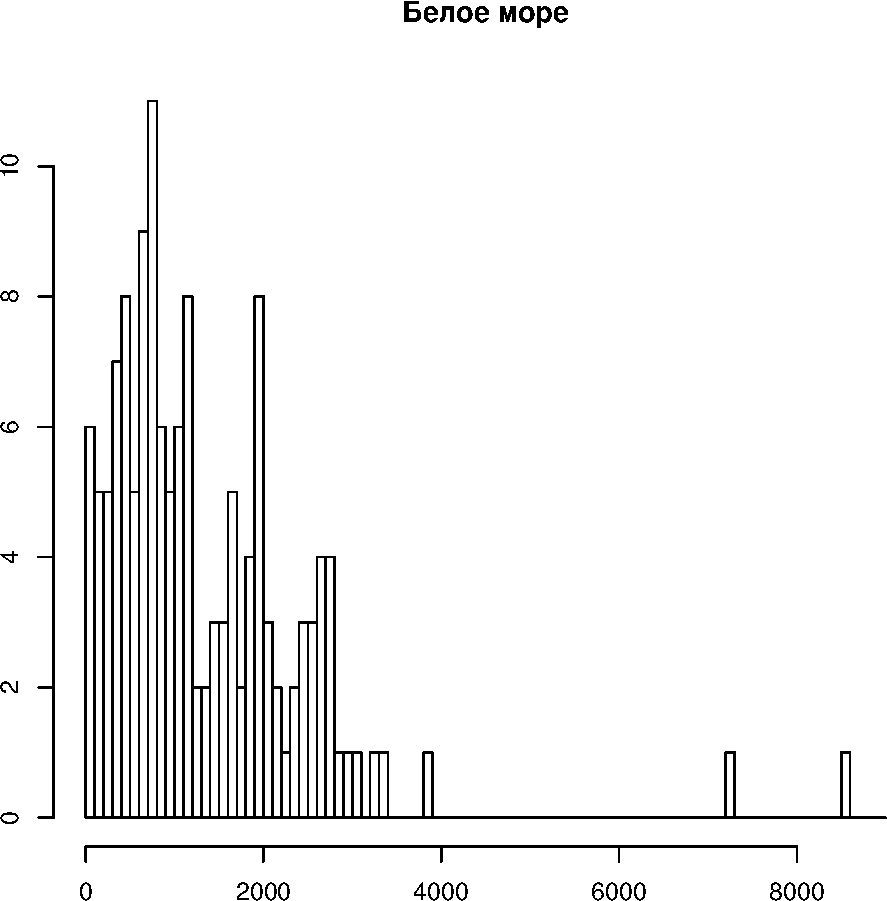
\includegraphics[height=.3\textheight]{../All_N/Nmean_hist_White.pdf}
		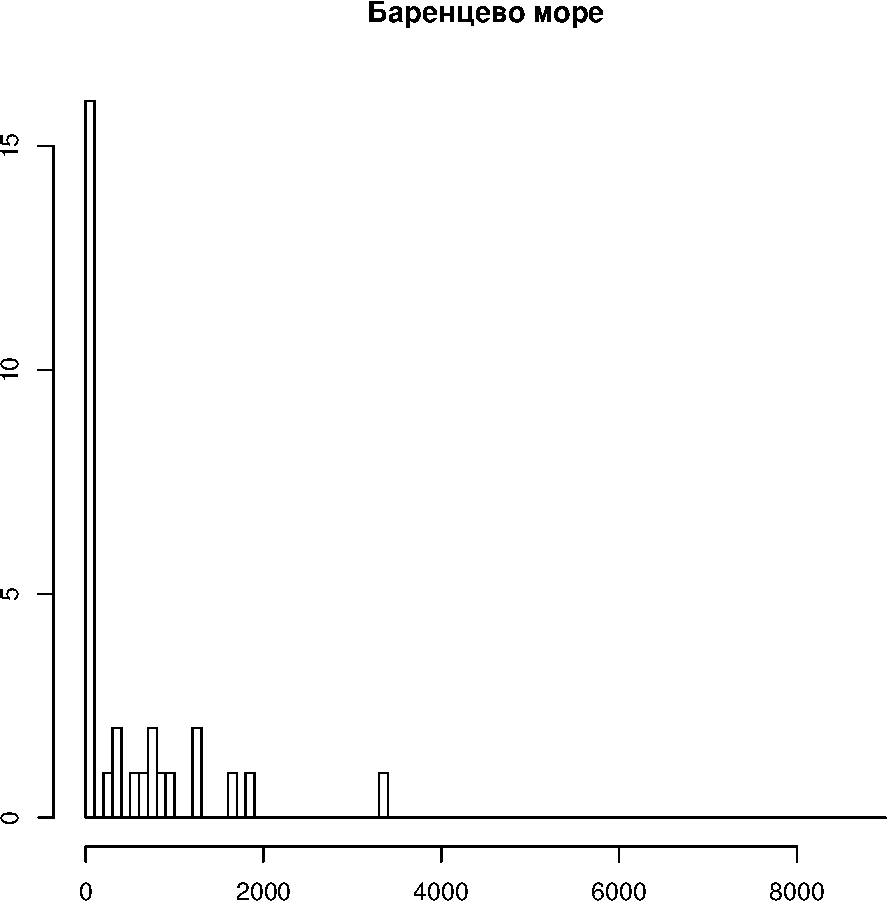
\includegraphics[height=.3\textheight]{../All_N/Nmean_hist_Barents.pdf}
	\caption{Частота встречаемости поселений с различным обилием {\it Macoma balthica}}
	{\footnotesize Примечание: по оси $X$ \textemdash средняя численность {\it Macoma balthica}, экз./м$^2$ (шаг \textemdash $100$~экз./м$^2$), по оси $Y$ 	\textemdash частота встречаемости}
	\label{ris:Nmean_hist}
	\end{figure}
%
Наиболее часто встречаются поселения со средней численностью $700-800$~экз./м$^2$.
Отдельные районы Кандалакшского залива Белого моря не отличались по средней численности маком ($Kruskal-Wallis\ \chi^2 = 5,6$, $p = 0,2$). 
При сравнении средних обилий маком на разных участках в пределах одного горизонта не показало достоверных отличий (табл.~\ref{tab:Nmean_Kruskal_mareography_White}).
%
	\begin{table}[ht]
	\caption{Сравнение среднего обилия {\it M.~balthica} в пределах одного мареографического уровня в Белом море}
	\label{tab:Nmean_Kruskal_mareography_White}
	\begin{tabular}{|*{4}{p{0.2\textwidth}|}} \hline
	ма\-ре\-ографи\-ческий уровень & $Kruskal-Wallis\ \chi^2$ & $df$ & $p$ \\
	\hline
	СГЛ & $2,7$ & $5$ & $0,7$ \\
	\hline
	НГЛ & $5,8$ & $4$ & $0,2$ \\
	\hline
	ноль глубин & $0,16$ & $1$ & $0,7$ \\
	\hline
	ВСЛ & $1$ & $1$ & $0,3$ \\
	\hline
	\end{tabular}

	{\footnotesize Примечания: градации мареографического уровня: ВГЛ \textemdash верхний горизонт литорали, СГЛ \textemdash средний горизонт литорали, НГЛ \textemdash нижний горидонт литорали, ВСЛ \textemdash верхняя сублитораль}
	\end{table}
%
    Сравнение средних численностей на разных горизонтах в пределах одного участка показало различные результаты (\ref{tab:N2_area_mareography_Kruskal_White}). 
%
	\begin{table}[ht]
	\caption{Сравнение обилия {\it M.~balthica} в поселених на разном мареографическом уровне в Белом море}
	\label{tab:N2_area_mareography_Kruskal_White}
        \begin{tabular}{|p{0.25\textwidth}|*{4}{p{0.15\textwidth}|}} \hline
    участок & $Kruskal-Wallis\ \chi^2$ & $df$ & $p$ & \\
	\hline
    Клющиха & $19,7$ & $2$ & $5,2 \times 10^{-05}$ & ***\\
    \hline
    Клющиха (только литораль) & $1,1$ & $1$ & $0,31$ & \\
    \hline
    Сухая & $0,0057$ & $1$ & $0,94$ & \\
    \hline
    Лисья & $17,5$ & $2$ & $0,00016$ & ***\\
    \hline
    Лисья (только литораль) & $11,06$ & $1$ & $0,00088$ & ***\\
    \hline
    Подпахта  & $2,3$ & $1$ & $0,13$ & \\
    \hline
    Горелый & $10,2$ & $3$ & $0,01658$ & ** \\
    \hline
    материк, Лувеньга & $2,4$ & $3$ & $0,50$ &  \\
    \hline
	\end{tabular}
    {\footnotesize Примечание: достоверность различий *** \textemdash $p<0,001$; ** \textemdash $p<0,05$; * \textemdash $p<0,1$.}
	\end{table}
%
Для участков в Сухой салме, проливе Подпахта, материковой литорали в Лувеньге варьирование численности между пробами перекрывало варьирование между горизонтами литорали.
При этом для участков в бухтах Клющиха и Лисья и на о.~Горелом Лувеньгских шхер  было показано достоверное влияние мареографического уровня на обилие маком. 
Интересно отметить, что в бухте Клющиха численность маком на нижнем и среднем горизонтах литорали не отличается ($403$~($7$)~экз./м$^2$), но в сублиторали она значительно выше ($1136$~($5$)~экз./м$^2$).
В бухте Лисья ситуация отличается, обилие маком на нижнем горизонте достоверно выше ($2832$~($10$)~экз./м$^2$), чем в среднем и в сублиторали ($1346$~($16$) и $1006$~($16$)~экз./м$^2$, соответсвенно). 



	\subsection{Баренцево море}

В Баренцевом море данные по обилию маком были получены для $12$ участков Мурманского побережья.
Минимальная средняя численность составляла $30$~экз./м$^2$ (г.~Дальнезеленецкая), что сравнимо с показателями для Белого моря. 
Максимальная средняя численность была значительно меньше, чем беломорская \textemdash $3350$~экз./м$^2$ (Абрам-мыс) (табл.~\ref{tab:mean_N_Barents}). 
	\begin{footnotesize}
	\begin{longtable}{|p{2cm}|p{3cm}|p{1cm}|p{2cm}|p{1.5cm}|p{1cm}|*{3}{c|}}
	\caption{Средняя численность {\it Macoma balthica} на различных участках Баренцева моря}\label{tab:mean_N_Barents}\\
	\hline
	Район & Участок & год & ма\-ре\-ографи\-ческий уровень & число повторностей & площадь учета & $N$, экз./м$^2$ & $S_x$  & $D, \%$ 
	\\ \hline \endfirsthead
	\hline
	\multicolumn{9}{|c|}{продолжение таблицы \ref{tab:mean_N_Barents}} \\ \hline
	Район & Участок & год & ма\-ре\-ографи\-ческий уровень & число повторностей & площадь учета & $N$, экз./м$^2$ & $S_x$  & $D, \%$ 
	\\ \hline \endhead
	\hline 
	\multicolumn{9}{|c|}{продолжение таблицы \ref{tab:mean_N_Barents} на следующей странице}
	\\ \hline \endfoot
	\endlastfoot
	Западный Мурман & Ура-губа & 2005 & СГЛ & 3 & 1/30 & 1267 & 288,8 & 23
		\\ \cline{2-9}
		 & Печенга & 2005 & СГЛ & 3 & 1/30 & 767 & 218,6 & 29
		\\ \hline
	Кольский Залив & Северное Нагорное & 2005 & СГЛ & 2 & 1/30 & 390 & 90,0 & 23
		\\ \cline{2-9}
		 & Абрам-мыс & 2005 & СГЛ & 2 & 1/30 & 3350 & 520,0 & 16
		\\ \cline{3-9}
		 &  & 2008 & СГЛ & 5 & 1/20 & 540 & 208,5 & 39
		\\ \cline{4-9}
		 &  &  & НГЛ & 5 & 1/20 & 1804 & 78,6 & 4
		\\ \cline{2-9}
		 & Ретинское & 2005 & СГЛ & 2 & 1/30 & 660 & 300,0 & 45
		\\ \cline{2-9}
		 & Пала-губа & 2007 & СГЛ & 16 & 1/30 & 936 & 76,4 & 8
		\\ \cline{3-9}
		 &  & 2007 осень & НГЛ & 36 & 1/30 & 790 & 61,7 & 8
		\\ \cline{3-9}
		 &  & 2008 зима & НГЛ & 11 & 1/20 & 864 & 154,4 & 18
		\\ \cline{3-9}
		 &  & 2008 & НГЛ & 10 & 1/30 & 1644 & 192,5 & 12
		\\ \hline
	Восточный Мурман & Гаврилово & 2008 & СГЛ & 5 & 1/30 & 138 & 20,3 & 15
		\\ \cline{4-9}
		 &  & 2008 & НГЛ & 5 & 1/30 & 24 & 11,2 & 47
		\\ \cline{2-9}
		 & Ярнышная & 2007 & СГЛ & 36 & 1/30 & 70 & 9,6 & 14
		\\ \cline{3-9}
		 &  & 2008 & ВГЛ & 5 & 1/30 & 414 & 47,8 & 12
		\\ \cline{4-9}
		 &  & & НГЛ & 5 & 1/30 & 387 & 109,1 & 28
		\\ \cline{2-9}
		 & Дальнезеленецкая & 2002 & СГЛ & 43 & 1/30 & 52 & 7,0 & 13
		\\ \cline{3-9}
		 &  & 2003 & СГЛ & 48 & 1/30 & 34 & 6,6 & 20
		\\ \cline{3-9}
		 &  & 2004 & СГЛ & 44 & 1/30 & 32 & 5,3 & 16
		\\ \cline{3-9}
		 &  & 2005 & СГЛ & 30 & 1/30 & 30 & 4,5 & 15
		\\ \cline{3-9}
		 &  & 2006 & СГЛ & 28 & 1/30 & 39 & 6,0 & 16
		\\ \cline{3-9}
		 &  & 2007 & СГЛ & 33 & 1/30 & 72 & 6,6 & 9
		\\ \cline{3-9}
		 &  & 2008 & СГЛ & 72 & 1/30 & 72 & 5,5 & 8
		\\ \cline{4-9}
		 &  &  & ВГЛ & 10 & 1/30 & 30 & 8,9 & 30
		\\ \cline{4-9}
		 &  &  & НГЛ & 5 & 1/30 & 42 & 7,3 & 17
		\\ \cline{2-9}
		 & Шельпино & 2008 & СГЛ & 5 & 1/30 & 54 & 11,2 & 21
		\\ \cline{4-9}
		 &  &  & ВГЛ & 5 & 1/30 & 36 & 17,5 & 49
		\\ \cline{2-9}
		 & Порчниха & 2007 & СГЛ & 32 & 1/30 & 87 & 10,8 & 12
		\\ \cline{3-9}
		 &  & 2008 & СГЛ & 5 & 1/30 & 60 & 13,4 & 22
		\\ \cline{2-9}
		 & Ивановская & 2008 & ВСЛ & 5 & 1/20 & 1208 & 72,8 & 6
		\\ \hline
	\multicolumn{9}{p{16cm}}{Примечания: градации мареографического уровня: ВГЛ \textemdash верхний горизонт литорали, СГЛ \textemdash средний 	горизонт литорали, НГЛ \textemdash нижний горидонт литорали, ВСЛ \textemdash верхняя сублитораль. 

	$N$, экз./м$^2$ \textemdash средняя численность {\it M.~balthica}. 
	$S_x$ \textemdash ошибка среднего.
	 $D, \%$ \textemdash  точность учета.
	
	В обозначении числа повторностей индекс ''и'' означает интегральную пробу, в этом случае в графе площадь учета указано сколько проб какой площади 	объединялись в одну.}
	\end{longtable}
	\end{footnotesize}
%
Среди иследованных, наиболее часто встречались поселения со средним обилием менее $100$~экз./м$^2$ (рис.~\ref{ris:N_region_Barents}).

Важно отметить, что для Мурманского побережья Баренцева моря показаны различия между отдельными районами: Западным, Восточным Мурманом и Кольским заливом. Это подтверждается нашими данными (рис.~\ref{ris:N_region_Barents}) по размаху варьирования среднего обилия в пределах районов ($Kruskal-Wallis\ \chi^2 = 17,6$, $p = 0,00015$).
%
	\begin{figure}[h]
		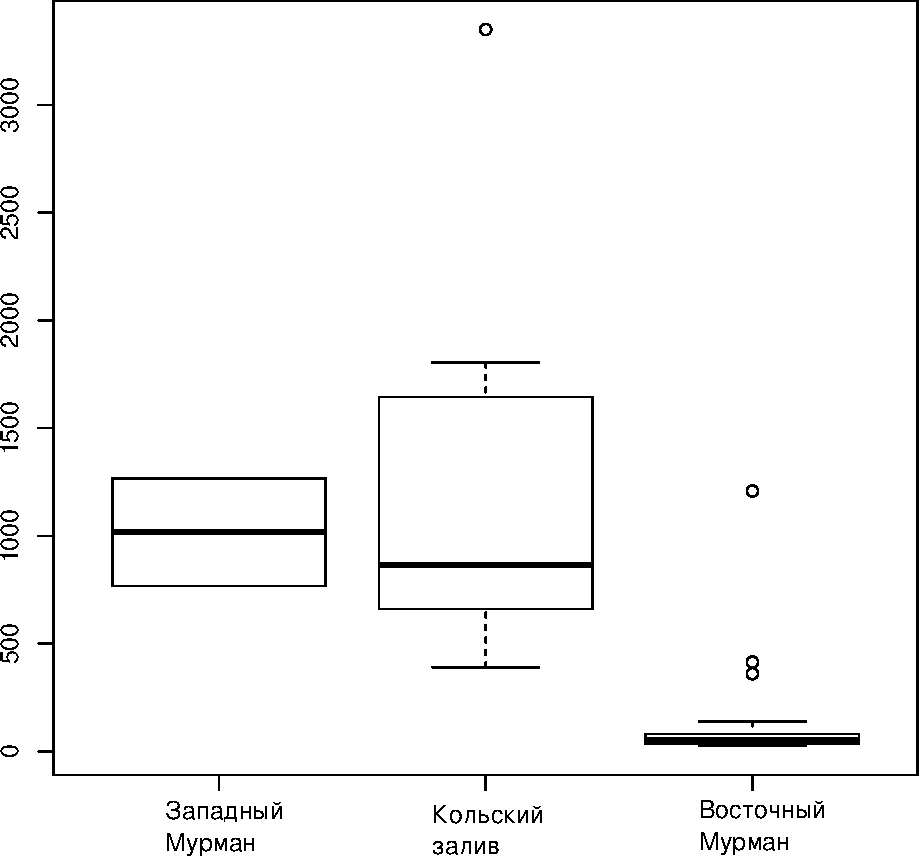
\includegraphics{../All_N/Nmean_region_Barents1.pdf}
	\caption{Варьирование среднего обилия {\it Macoma balthica} в разных районах Мурманского побережья Баренцева моря}
	{\footnotesize Примечание: По оси абсцисс \textemdash численность {\it M.~balthica}, ~экз./м$^2$.

	На графике: жирная горизонтальная линия \textemdash медиана, границы ''ящика'' \textemdash 1 и 3 квартили, ''усы'' \textemdash $1,5$ интерквартильного расстояния, точки - значения выпадающие за $1,5$ интерквартильных расстояния}
	\label{ris:N_region_Barents}
	\end{figure}
%
На литорали Восточного Мурмана численность {\it M.~balthica} в основном не превышала $100$~экз./м$^2$. 
Единственное исключение \textemdash\ литораль губы Ярнышная, где численность маком достигала $410$~($12$)~экз./м$^2$. 
Между тем, на единственном участке, где были учеты в сублиторали, в губе Ивановской, численность на порядок выше, чем ее значения на литорали Восточного мурмана, и составляет $1200$~экз./м$^2$. 
В Кольском заливе минимальные значения обилия были отмечены на литорали в районе Северного Нагорного ($390$~($23$)~экз./м$^2$). 
Максимальных значений численности как для региона, так и для всей исследованной части Мурманского побережья, достигали поселения маком на учатске в районе Абрам-мысса ($3350$~($16$)~экз./м$^2$). 
На Западном Мурмане обилие флуктуировало вокруг $1000$~экз./м$^2$.  

При сравнении численности маком на различных мареографических уровнях различия между горизонтами литорали были показаны для губ Гаврилово и Ярнышная (табл.~\ref{tab:N2_area_mareography_Kruskal_Barents}).
В Гаврилово средняя численность {\it M.~balthica} в среднем горизонте литорали превышала аналогичные значения для нижнего горизонта на порядок ($138$~($15$) и $24$~($47$)~экз./м$^2$, соответственно.
В губе Ярнышная численность маком в верхнем и нижнем горизонтах не различалась ($414$~($12$) и $360$~($43$)~экз./м$^2$, соответсвенно), в то время как в среднем горизонте литорали она была значительно ниже ($70$~($14$)~экз./м$^2$).  
%
	\begin{table}[ht]
	\caption{Сравнение обилия {\it Macoma balthica} в поселених на разном мареографическом уровне в Баренцевом море}
	\label{tab:N2_area_mareography_Kruskal_Barents}
        \begin{tabular}{|p{0.25\textwidth}|*{4}{p{0.15\textwidth}|}} \hline
    Абрам-мыс &  $1,5$ & $1$ & $0,224$ & \\
    \hline
    Пала-губа & $0,4$ & $1$ & $0,54$ & \\
    \hline
    Гаврилово & $6,9$ & $1$ & $0,0084$ & *** \\
    \hline
    Ярнышная & $19,4$ &  $2$ &  $6,09 \times 10^{-5}$ & *** \\
    \hline
    Дальнезеленецкая & $1,6$ & $2$ & $0,45$ & \\
    \hline
    Шельпино & $0,7$ & $1$ & $0,39$ & \\
    \hline
	\end{tabular}
    {\footnotesize Примечание: достоверность различий *** \textemdash $p<0,001$; ** \textemdash $p<0,05$; * \textemdash $p<0,1$.}
	\end{table}
%

    \subsection{Влияние состава грунта на численность {\it Macoma balthica}}
Нет сомнений, что основной параметр, определяющий обилие маком \textemdash\ это доступные пищевые   ресурсы.   
Косвенным   показателем   наличия   пищевых   ресурсов   служит гранулометрический состав грунта и общее содержание органических веществ. 
Поэтому мы провели корреляционный анализ связи среднего обилия маком на участке с характеристиками  грунта.  
В   результате  оказалось,   что   соотношение   песчаных   фракций   различного   размера влияет   на   обилие  {\it M.~balthica}  (\ref{}).  
%

%
При   этом  наблюдается   достоверная   отрицательная корреляция численности маком с долей крупного  песка и положительная — с долей мелкого.

\end{document}
